\documentclass[a4paper,11pt]{article}
\input{/home/tof/Documents/Cozy/latex-include/preambule_doc.tex}
\input{/home/tof/Documents/Cozy/latex-include/preambule_commun.tex}
\newcommand{\showprof}{show them}  % comment this line if you don't want to see todo environment
\setlength{\fboxrule}{0.8pt}
\fancyhead[L]{\fbox{\Large{\textbf{Algo 20}}}}
\fancyhead[C]{\textbf{Exercices parcours graphe}}
\newdate{madate}{10}{09}{2020}
%\fancyhead[R]{\displaydate{madate}} %\today
\fancyhead[R]{Terminale - NSI}
\fancyfoot[L]{\vspace{1mm}Christophe Viroulaud}
\AtEndDocument{\label{lastpage}}
\fancyfoot[C]{\textbf{Page \thepage/\pageref{lastpage}}}
\fancyfoot[R]{\includegraphics[width=2cm,align=t]{/home/tof/Documents/Cozy/latex-include/cc.png}}

\begin{document}
\begin{exo}
    \begin{center}
        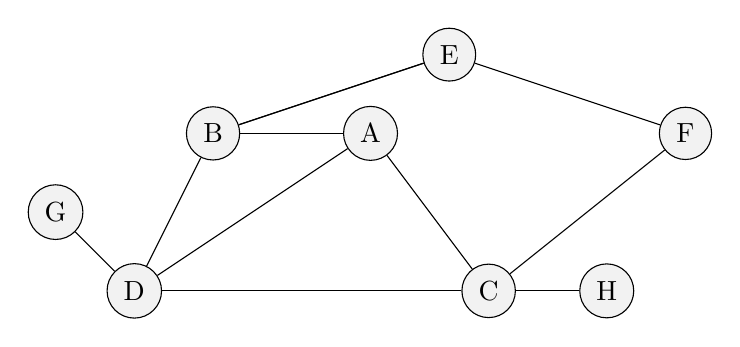
\begin{tikzpicture}
            \node[draw,circle,fill=gray!10] (A)at(0,2) {A};
            \node[draw,circle,fill=gray!10] (B)at(-2,2) {B};
            \node[draw,circle,fill=gray!10] (C)at(1.5,0) {C};
            \node[draw,circle,fill=gray!10] (D)at(-3,0) {D};
            \node[draw,circle,fill=gray!10] (E)at(1,3) {E};
            \node[draw,circle,fill=gray!10] (F)at(4,2) {F};
            \node[draw,circle,fill=gray!10] (G)at(-4,1) {G};
            \node[draw,circle,fill=gray!10] (H)at(3,0) {H};
            \draw[-,>=latex] (A) -- (B);
            \draw[-,>=latex] (A) -- (C);
            \draw[-,>=latex] (A) -- (D);
            \draw[-,>=latex] (D) -- (B);
            \draw[-,>=latex] (B) -- (E);
            \draw[-,>=latex] (B) -- (E);
            \draw[-,>=latex] (D) -- (G);
            \draw[-,>=latex] (C) -- (F);
            \draw[-,>=latex] (C) -- (H);
            \draw[-,>=latex] (C) -- (D);
            \draw[-,>=latex] (E) -- (F);
        \end{tikzpicture}
    \end{center}
    \begin{enumerate}
        \item Donner l'ordre du graphe.
        \item Donner le degré du sommet D.
        \item Reprendre le parcours en profondeur vu en classe (code \ref{cours}) et remplacer le tableau \textbf{\texttt{visites}} par un dictionnaire associant chaque sommet à un booléen.
    \begin{lstlisting}[language=Python  , xleftmargin=2em, xrightmargin=2em]
def profondeur(graphe: dict, noeud: str, visites: list) -> None:
    if noeud not in visites:
        print(noeud, end=" ")
        visites.append(noeud)
        for voisin in graphe[noeud]:
            profondeur(graphe, voisin, visites)
\end{lstlisting}
              \captionof{code}{Parcours en profondeur vu en cours}
              \label{cours}
        \item Étudier la complexité temporelle
    \end{enumerate}

\end{exo}
\end{document}